\documentclass[14pt]{article}
\usepackage{geometry}
\usepackage[utf8]{inputenc}
\usepackage{cmap}
\usepackage[russian]{babel}
\usepackage{textcomp}
\usepackage{indentfirst}
\usepackage{amssymb}
\usepackage{graphicx}
\usepackage{lipsum}
\usepackage{setspace}
\usepackage{extsizes}
\usepackage{enumitem}
\usepackage{tabularx}
\usepackage{amsmath}
\usepackage{tocloft}
\usepackage{minted}
\usepackage[colorlinks=true,urlcolor=blue,linkcolor=]{hyperref}

\usepackage{graphicx}
\graphicspath{ {./images/} }

\renewcommand{\cftsecleader}{\cftdotfill{\cftdotsep}}
\renewcommand{\cfttoctitlefont}{\LARGE\bfseries}
% Начало блока кода, который позволяет включить section* в оглавление
\usepackage{etoolbox}
\makeatletter
\newcommand\mysection[1]{%
	  \addcontentsline{toc}{section}{#1}%
	  \section*{#1}%
}
\makeatother

\makeatletter
\newcommand\mysubsection[1]{%
	  \addcontentsline{toc}{subsection}{#1}%
	  \subsection*{#1}%
}
\makeatother

\makeatletter
\newcommand\mysubsubsection[1]{%
	  \addcontentsline{toc}{subsubsection}{#1}%
	  \subsubsection*{#1}%
}
\makeatother
% Конец блока кода

\usepackage{titlesec}
\titleformat*{\section}{\LARGE\bfseries\centering}
\titleformat*{\subsection}{\Large\it}
\usepackage{pgfplots}

\newcolumntype{Y}{>{\centering\arraybackslash}X}

\begin{document}
\newgeometry{top=0.1in,bottom=0in,right=0.1in,left=0.1in}
\begin{spacing}{1}
\begin{center}
	\makebox[\linewidth][s]{МИНИСТЕРСТВО НАУКИ И ВЫСШЕГО ОБРАЗОВАНИЯ РОССИЙСКОЙ ФЕДЕРАЦИИ} \\
	\vspace{5mm}
	ФЕДЕРАЛЬНОЕ ГОСУДАРСТВЕННОЕ АВТОНОМНОЕ ОБРАЗОВАТЕЛЬНОЕ \\ УЧРЕЖДЕНИЕ ВЫСШЕГО ОБРАЗОВАНИЯ  \\
	\guillemotleft Национальный исследовательский университет ИТМО\guillemotright \\
	\vspace{5mm}
	ФАКУЛЬТЕТ ПРОГРАММНОЙ ИНЖЕНЕРИИ И КОМПЬЮТЕРНОЙ ТЕХНИКИ
	\vspace{60mm}
	
	{\bf \LARGE ЛАБОРАТОРНАЯ РАБОТА №1} \\
	{ \Large по дисциплине \\
	\guillemotleft Системы искусственного интелекта \guillemotright \\}
\end{center}
\vspace{50mm}

\begin{flushright}
	{\it \textbf{Выполнил работу:}}\\
	Студент группы P3318 \\
	Рамеев Тимур Ильгизович \\
	{\it \textbf{Преподаватель:}}\\
	Авдюшина Анна\\
	Евгеньевна \\
\end{flushright}
\vspace{18mm}
\end{spacing}
\begin{center}
    Санкт-Петербург  2024
\end{center}

\newgeometry{a4paper, top=10mm, bottom=20mm, left=20mm, right=10mm}

\newpage
\begin{center}
	\tableofcontents 
\end{center}
\setcounter{page}{1}

\newpage
\mysection{Цель}
	Знакомство с базами знаний и онтологиями, языком Prolog и редактором онтологий Protege.
\mysection{Основные концепции и инструменты}
	В основе баз знаний лежат факты и правила. Факты представляют из себя верные отношения между сущностями, а правила - способы порождения новых фактов из имеющихся. \\
	Для использования базы знаний необходимо задать цель - неизвестную переменную в предикате, которую база попытается подобрать так, чтобы предикат был верен. \\
	Язык Prolog позволяет описать базу занний декларативно. В нем можно описать факты - верные предикаты с полными аргументами, а также задать аналоги функций - правила.
\mysection{Описание базы знаний}
	База знаний, написанная на языке Prolog, содержит информацию о персонажах вселенной League Of Legends. В ней описаны класс персонажа, его роль на карте, место обитания (по лору), а также враждебные отношения между персонажами (по лору).
	Также база знаний содержит следующие правила:
	\begin{enumerate}[itemsep=-5pt]
		\item Правило для поиска персонажей с одной территории
		\item Правило для поиска персонажей с одинаковой ролью
		\item Правило, ищущее всех топеров-стрелков
		\item Правило для поиска войны между территориями
		\item Правило для поиска врагов с одинаковой ролью на карте
		\item Правило для поиска друзей (Территории с общим врагом без войны друг с другом)
	\end{enumerate}

\newpage
\mysection{Запросы к базе знаний}
	Помимо базы знаний, были написаны несколько запросов к ней, для демонстрации ее работы:
	\begin{enumerate}[itemsep=-5pt]
		\item Посмотреть всех убийц
		\item Посмотреть с какой территории песонаж Трэш
		\item Посмтотреть есть ли враги у Ка'Зикса
		\item Посмтотреть магов из Бандл-Сити, играющих на топе или на миде
		\item Посмотреть всех врагов Ноксуса
		\item Посмотреть всех воинов и убийц играющих против магов на одной позиции
	\end{enumerate}


\mysection{Программная часть}
\mysubsection{База знаний}
\begin{minted}[mathescape, linenos]{prolog}
% Роль персонажа
tank(tarik).
tank(trash).
tank(braum).
wizard(zerat).
wizard(ari).
wizard(sweyn).
wizard(reykan).
wizard(veigar).
wizard(luxe).
warrior(vai).
warrior(viego).
warrior(darius).
warrior(saylas).
warrior(warwick).
warrior(garen).
killer(khaZix).
killer(rengar).
killer(pyke).
killer(zed).
killer(ekko).
killer(katarina).
shooter(timo).
shooter(ashe).
shooter(senna).
shooter(lucian).
shooter(dreivan).
shooter(jinx).

% Родина персонажа ( по лору )
homeland(shadowyIslands, lucian).
homeland(shadowyIslands, senna).
homeland(shadowyIslands, viego).
homeland(shadowyIslands, trash).
homeland(gapingHole, khaZix).
homeland(bildgwater, pyke).
homeland(ionia, zed).
homeland(ionia, rengar).
homeland(ionia, reykan).
homeland(nocsus, sweyn).
homeland(nocsus, dreivan).
homeland(nocsus, darius).
homeland(nocsus, katarina).
homeland(zaun, jinx).
homeland(zaun, vai).
homeland(zaun, ekko).
homeland(zaun, warwick).
homeland(demasiya, luxe).
homeland(demasiya, garen).
homeland(freljord, saylas).
homeland(freljord, ashe).
homeland(freljord, braum).
homeland(targon, tarik).
homeland(bandlCity, veigar).
homeland(bandlCity, timo).
homeland(bandlCity, ari).
homeland(shurima, zerat).


% Место отыгрыша на карте (Некорректно немного получилось)
role(carry, lucian).
role(support, trash).
role(support, senna).
role(jungle, viego).
role(jungle, khaZix).
role(support, pyke).
role(mid, zed).
role(jungle, rengar).
role(support, reykan).
role(support, sweyn).
role(carry, dreivan).
role(top, darius).
role(carry, jinx).
role(jungle, vai).
role(jungle, ekko).
role(jungle, warwick).
role(mid, luxe).
role(top, garen).
role(mid, saylas).
role(carry, ashe).
role(support, braum).
role(support, tarik).
role(mid, veigar).
role(top, timo).
role(mid, ari).
role(mid, zerat).
role(mid, katarina).

% Враги (по лору )
enemies(khaZix, rengar).
enemies(saylas, garen).
enemies(garen, darius).
enemies(katarina, ari).
enemies(timo, pyke).
enemies(senna, trash).
enemies(senna, viego).
enemies(lucian, trash).
enemies(lucian, viego).
enemies(jinx, vai).

% Персонажи с одной территории
countrymans(X, Y) :- homeland(Z, X), homeland(H, Y), Z = H, X \= Y.

% Персонажи с одинаковой ролью
sameRoles(X, Y) :- role(Z, X), role(H, Y), Z = H, X \= Y.

% Топеры-стрелки
topShooters(X) :- role(top, X), shooter(X).

% Войны между территориями
wars(X, Y) :- homeland(X, Z), homeland(Y, H), (enemies(Z, H); enemies(H, Z)), X \= Y.

% Враги с одинаковой позицией в игре
sameEnemiesByRole(X, Y) :- role(Z, X), role(H, Y), (enemies(X, Y); enemies(Y, X)), X \= Y, Z = H.

% Друзья (Территории с общим врагом без войны друг с другом)
friends(X, Y) :- wars(X, Z), wars(Y, Z), not(wars(X, Y)), X \= Y.
\end{minted}

\mysubsection{Запросы к базе знаний}
\begin{minted}[mathescape, linenos]{prolog}
% посмотреть всех убийц
killer(X).

% посмотреть с какой территории Треш
homeland(X,trash).

% посмотреть, есть ли враги у казикса
enemies(khaZix, _); enemies(_, khaZix).

% посмотреть магов из Бандл-Сити, играющих на топе или на миде
wizard(X), homeland(bandlCity, X), (role(top, X); role(mid, X)).

% посмотреть всех врагов Ноксуса
{Z}/(wars(nocsus, Y), homeland(Y, Z)).

% посмотреть всех воинов и убийц играющих против магов на одной линии
(killer(X); warrior(X)), wizard(Y), role(Role, X), role(Role, Y).
\end{minted}


\mysection{Онтологический граф}
\begin{center}
	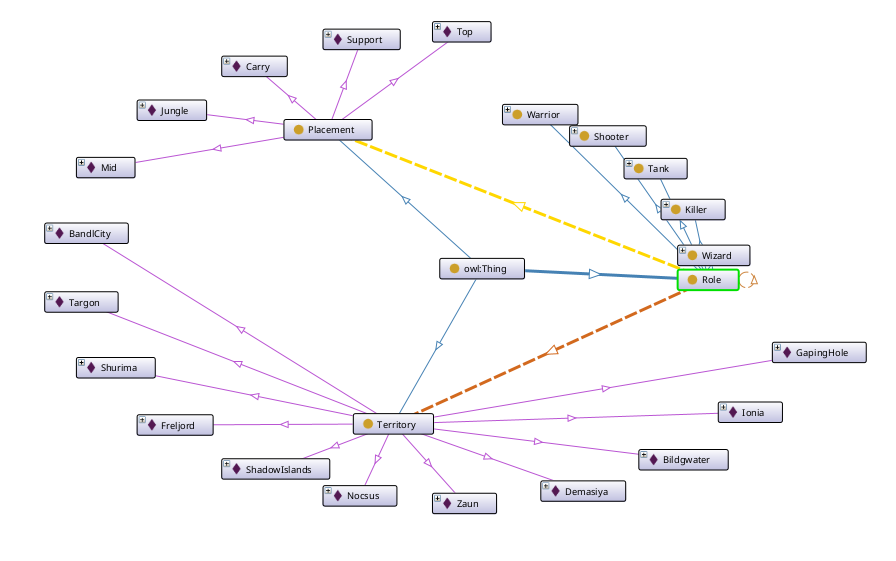
\includegraphics[scale=0.6]{onto_graph}
\end{center}

\newpage
\mysection{Вывод}
Мы познакомились с основными концепциями баз знаний и онтологий, освоили язык Prolog и редактор онтологий Protege. Базы знаний на Prolog позволяют удобно осуществлять резолюцию целей по имеющимся фактам, а система Protege может выявлять несоотвестивия и "скрытую информацию" в разработанных онтологиях.
\end{document}